\documentclass{easychair}

% \usepackage{doc}
\usepackage{setspace}
\usepackage{verbatim}
\usepackage{amssymb}
\usepackage{wasysym}
\usepackage[straightquotes]{newtxtt}


%----Making things more compact
%----Suppress extra space in texttt mode
%\AddToHook{cmd/ttfamily/after}{\frenchspacing}
% \newcommand{\smalltt}[1]{\small \texttt{#1}}

\newenvironment{packed_itemize}{
\vspace*{-0.3em}
\begin{itemize}
\setlength{\partopsep}{0pt}
\setlength{\itemsep}{1pt}
\setlength{\parskip}{0pt}
\setlength{\parsep}{0pt}
}{\end{itemize}}
\newenvironment{packed_enumerate}{
\vspace*{-0.3em}
\begin{enumerate}
\setlength{\partopsep}{0pt}
\setlength{\itemsep}{1pt}
\setlength{\parskip}{0pt}
\setlength{\parsep}{0pt}
}{\end{enumerate}}
% \renewcommand{\textfraction}{0.07}
% \renewcommand{\topfraction}{0.9}
% \renewcommand{\bottomfraction}{0.9}
% \renewcommand{\floatpagefraction}{0.66}
% \setlength{\floatsep}{2.0pt plus 2.0pt minus 2.0pt}
% \setlength{\textfloatsep}{5.0pt plus 2.0pt minus 0.0pt}

\newcommand{\dav}[1]{{\color{red}{David: {#1}}}}
\newcommand{\jack}[1]{{\color{red}{Jack: {#1}}}}

\title{Towards StarExec in the Cloud}

\author{
  David Fuenmayor\inst{1}
\and
  Jack McKeown\inst{2}
\and
  Geoff Sutcliffe\inst{2}
}

\institute{
  University of Bamberg,
  Bamberg, Germany\\
  \email{david.fuenmayor@uni-bamberg.de}
\and
  University of Miami,
  Miami, USA\\
  \email{jam771@miami.edu,geoff@cs.miami.edu}
}

\authorrunning{Fuenmayor, McKeown, Sutcliffe}
\titlerunning{Stars in the Clouds}

\begin{document}
\maketitle

%--------------------------------------------------------------------------------------------------
\begin{abstract}
StarExec has been central to much progress in logic solvers over the last 10 years.
It was recently announced that StarExec Iowa will be decommissioned, and while StarExec Miami 
will continue to operate while funding is available, it will not be able to support the large 
number of logic solver communities supported by the larger StarExec Iowa. 
In the long term StarExec will necessarily have to migrate to a commonly available compute 
service. 
This paper describes work being done to reengineer StarExec as a cloud-native application using
container technology and infrastructure-as-code practices.
The first step has been to containerize StarExec and ATP systems so that they can be run on a 
broad range of computer platforms. 
The next step in process is to write a new backend in StarExec so that Kubernetes can be used to 
orchestrate distribute of StarExec job pairs over whatever compute nodes are available.
FIX HERE One possibility is to host StarExec-Kubernetes in AWS.
\end{abstract}
%--------------------------------------------------------------------------------------------------
% Geoff
\section{Introduction}
\label{Introduction}

Automated Theorem Proving (ATP) is concerned with the development and use of tools that automate 
sound reasoning: the derivation of conclusions that follow inevitably from facts.
Automated Theorem Proving (ATP) is at the heart of many computational tasks, in particular for
verification \cite{Har06,HH19} and security \cite{Coo18}.\footnote{%
In AWS -
\href{https://aws.amazon.com/what-is/automated-reasoning/}{\tt aws.amazon.com/what-is/automated-reasoning/}, 
\href{https://aws.amazon.com/security/provable-security//}{\tt aws.amazon.com/security/provable-security/}.} 
New and emerging application areas include
chemistry \cite{Yad17}, 
biology \cite{CC+13}, 
medicine \cite{HLB05},
elections \cite{Nip09,BDS17}, 
auctions \cite{CK+15}, 
privacy \cite{Lib20},
law \cite{PS15}, 
ethics \cite{DF+16}, 
religion \cite{OZ11,BW14-ECAI,Hor19},
and business \cite{Han98}.
ATP systems are also used as components of more complex Artificial Intelligence (AI) systems,
and the impact of ATP is thus extended into many facets of society.
% in areas such as 
% knowledge representation \cite{TR+04}, 
% natural language processing \cite{BM05}, 
% planning \cite{NV07}, 
% agents \cite{TBP03}, 
% commonsense reasoning \cite{MS05}, 
% and the semantic web \cite{McG04}.

The Thousands of Problems for Theorem Provers (TPTP) World \cite{Sut24} is a well established 
infrastructure that supports research, development, and deployment of ATP systems.
The TPTP World includes 
the TPTP problem library \cite{Sut17},
the TSTP solution library \cite{Sut10},
standards for writing ATP problems and reporting ATP solutions \cite{SS+06,Sut08-KEAPPA},
tools and services for processing ATP problems and solutions \cite{Sut10},
and it supports the the annual CADE ATP System Competition (CASC)~\cite{Sut16}.
Since its first release in 1993 the ATP community has used the TPTP World as an appropriate and 
convenient infrastructure for ATP system development, evaluation, and application.
The TPTP World has a diverse, engaged, and sustained user community, with various parts of the 
TPTP World being deployed in a range of applications in both academia and industry.\footnote{%
TPTP has contributed to recognized research in 627 publications that cite \cite{Sut17},
according to Google Scholar.}
The web page \href{https://www.tptp.org}{\tt www.tptp.org} provides access to all components.

The TPTP problem library was motivated by the need to provide support for meaningful ATP system 
evaluation.
This need was also (or became) evident in other logic solver communities, e.g., 
SAT~\cite{HS00-SATLIB} and SMT~\cite{BST10}.
For many years testing of logic solvers was done on individual developer's computers. 
In 2010 a proposal for centralised hardware and software support was developed,
and in 2011 a \$2.11 million NSF grant\footnote{%
NSF Awards 1058748 and 1058925, led by Aaron Stump and Cesare Tinelli at the University of Iowa} 
was obtained.
This grant led to the development and availability of StarExec Iowa~\cite{SST14} in 2012,
and a subsequent \$1.00 million grant\footnote{%
NSF Award 1730419} in 2017 expanded StarExec to Miami.
StarExec has been central to much progress in logic solvers over the last 10 years, supporting
16 logic solver communities, used for running many annual competitions~\cite{BB+19}, and 
supporting many many users.
StarExec Iowa provides community infrastructure for many logic solver communities,
e.g., ASP, QBF, SAT, SMT, Termination, etc, while
StarExec Miami is used by the TPTP community.
StarExec Miami has features that take advantage of TPTP standards, and is also used to host CASC.

It was recently announced that StarExec Iowa will be decommissioned. 
The maintainer of StarExec Iowa explained that ``the plan is to operate StarExec as usual for 
competitions Summer 2024 and Summer 2025, and then put the system into a read-only mode for one 
year (Summer 2025 to Summer 2026)''.
The 2017 grant for StarExec Miami paid for the hardware and three years of system administration.
The hardware is still hosted by the University of Miami High Performance Computing group,
funded on a shoe-string budget by the TPTP World.
While StarExec Miami will continue to operate while funding is available, it will not be able
to support the large number of logic solver communities supported by the larger StarExec Iowa.
In the long term StarExec will necessarily have to migrate to a commonly available compute service.
This paper describes work being done to reengineer StarExec as a cloud-native application using
container technology and infrastructure-as-code practices.
The first step has been to containerize\footnote{%
Strictly, ``images'' are built, and the images are deployed in containers. 
But keeping with common use of the terminology, we just say ``container'' and ``containerize''.} 
StarExec and ATP systems so that they can be run on a broad range of computer platforms.
The next step in process is to write a new backend in StarExec so that Kubernetes can be used to
orchestrate distribute of StarExec job pairs over whatever compute nodes are available.
Additionally, this work aims to build a Kubernetes backend in StarExec so that Kubernetes can
be used to orchestrate distribute of StarExec job pairs over whatever compute nodes are available.
Supported by an Amazon Research Award (see Section~\ref{StarExecK}) a new version of StarExec
will be deployed in AWS.
This StarExec instance will be fully functional and available to the community (as much as our 
budget allows). 
It will also serve as an exemplary implementation for those willing to deploy their own, possibly 
customized, StarExec on their own computers or in the cloud.

\paragraph{This paper is organized as follows:}
Section~\ref{Background} provides a short background to ATP systems, StarExec, and 
containerization.
Section~\ref{ContainerizingStarExec} describes how StarExec has been containerized, and
Section~\ref{ContainerizingATPSystems} describes how ATP systems have been containerized.
Section~\ref{StarExecK} explains how we plan to deploy the containerized StarExec
and ATP systems in a Kubernetes setting.
Section~\ref{Conclusion} concludes and look forward to future work.

%--------------------------------------------------------------------------------------------------
\section{Background}
\label{Background}

%--------------------------------------------------------------------------------------------------
\subsection{ATP Systems}
\label{ATPSystems}

ATP Systems are complex pieces of software, typically using advanced data structures~\cite{Sch13}, 
sophisticated algorithms~\cite{Vor01}, and tricky code optimizations\cite{Sch06}.
They are written in a variety of programming languages: Prolog~\cite{Ott23,Hol23}, 
Scala~\cite{SB18}, C~\cite{SCV19}, C++~\cite{RV02-AICOMM}, OCaml~\cite{Kor06}, Python~\cite{SP20}, 
etc.
Their build processes include techniques such as parser generators~\cite{Ste21}, Makefiles,
code repositories, specific versions of libraries, etc.
For a user who is focussed on an application of ATP
% , e.g. (with a few exemplar references), in 
% mathematics \cite{Qua92-Book,MP96}, logic~\cite{GO86,Jec95}, management~\cite{PB+92-TR,PM94}, 
% planning \cite{SE94}, 
installing an ATP system can be a deal breaker, and many early users selected a weaker system, 
e.g., Otter~\cite{McC03-Otter}, for their experiments because it was readily available and easy 
enough to install.
% As the TPTP World evolved it was clear that more powerful ATP systems were available, especially
% evident in the CADE ATP System Competition (CASC)~\cite{Sut16}.
% However, these more powerful systems were often not as easy to obtain and install.
% This was a key motivation for the creation of the SystemOnTPTP service~\cite{Sut00-CADE-17}.
% SystemOnTPTP allows users to
% The ATP systems in SystemOnTPTP are installed by the third author, often with help from the
% individual system developers.
There have been some proposals for standardising the ATP system build process, e.g.,
\href{https://tptp.org/Proposals/SystemBuild.html}{\tt tptp.org/Proposals/SystemBuild.html}, 
but the diversity of ATP system software makes conformity nigh impossible.
An alternative is to push the task back on the system developers, and one approach to this is
containerizing the ATP systems, as discussed in Section~\ref{Containerization}.

%--------------------------------------------------------------------------------------------------
\subsection{StarExec}
\label{StarExec}

The need to provide support for meaningful system evaluation has been recognized in many logic 
solver communities, e.g., TPTP~\cite{SS01}, SAT~\cite{HS00-SATLIB}, SMT~\cite{CSW15},
Termination~\cite{MZ07}, etc.
For many years testing of logic solvers was done on individual developer's computers. 
In 2010 a proposal for centralised hardware and software support was developed,
and in 2011 a \$2.11 million NSF grant\footnote{%
NSF Awards 1058748 and 1058925, led by Aaron Stump and Cesare Tinelli at the University of Iowa} 
was obtained.
This grant led to the development and availability of StarExec Iowa~\cite{SST14} in 2012,
and a subsequent \$1.00 million grant\footnote{%
NSF Award 1730419} in 2017 expanded StarExec to Miami.
StarExec has been central to much progress in logic solvers over the last 10 years, supporting
16 logic solver communities, used for running many annual competitions~\cite{BB+19}, and 
supporting many many users.

Figure~\ref{ArchitectureS} shows the architecture of the currently deployed StarExec.
The hardware consists of a single head node and multiple compute nodes.
The head node provides the browser interface for users, in particular it accepts job requests
that generate job pairs consisting of an ATP system and a problem file, does internal scheduling,
and uses the SUN Grid Engine (SGE) cluster management to distribute the pairs to the compute nodes.
(For development and testing, the head node can also run job pairs itself using a local backend.)
The head node maintains a relational MariaDB database, and all the nodes access an NFS mounted
shared file system.
The database records everything, including the ATP systems' files and the problem files in the 
file system. \jack{My understanding is that many things like the benchmarks and solvers are not stored in mariadb, but are just on disk on the head node and get copied to NFS directories when they're needed by job pairs on the compute nodes. I think paths to them are stored in mariadb though. That's probably what you meant, but to me the previous sentence sounded like it was saying benchmarks/solvers are stored in the database.}
Job pairs executing on a compute node have their time and memory usage limited and reported
by the {\tt runsolver}~\cite{Rou11} utility (the {\tt BenchExec}~\cite{BLW19} utility in 
StarExec Iowa).
The results and resource usage data from completed job pairs are stored in the file system, 
and recorded in the database.
The browser interface provides the necessary facilities to upload ATP systems, upload problem
files, browse the ATP systems and problems, create jobs, track job progress, browse and download
job results, and delete ATP systems, problems, jobs, etc. \jack{Also for creating users and controlling their resource limits and permissions}

\begin{figure}[htb]
\begin{center}
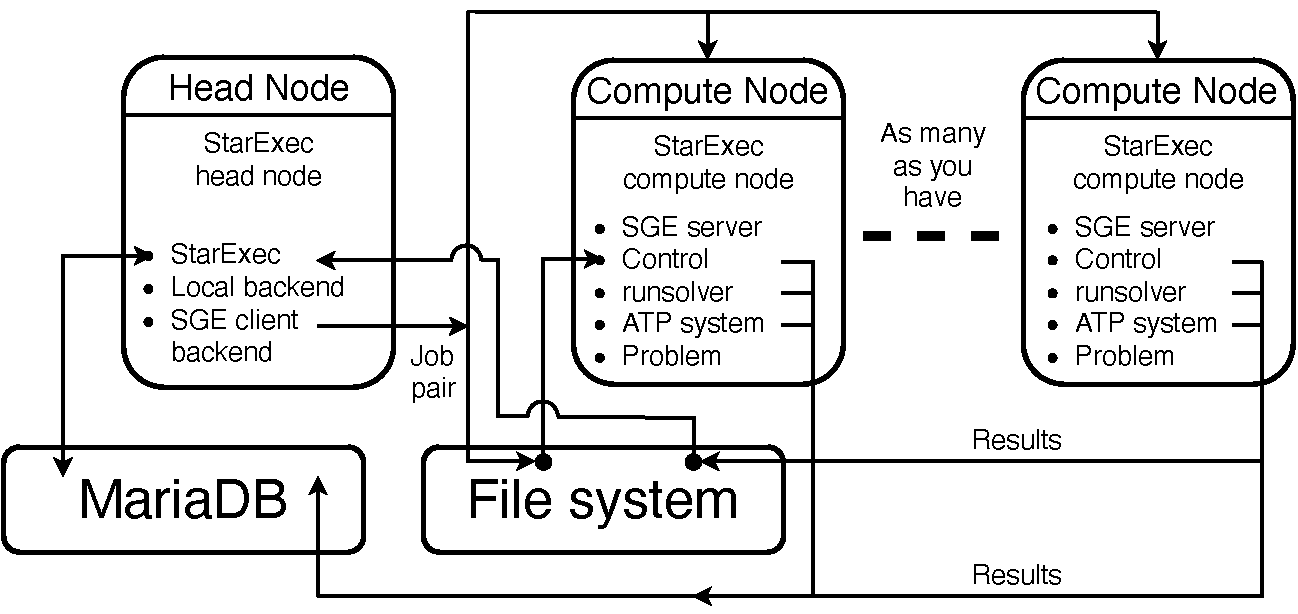
\includegraphics[width=0.8\textwidth]{ArchitectureS}
\caption{StarExec Architecture}
\label{ArchitectureS}
\end{center}
\end{figure}

It was recently announced that StarExec Iowa will be decommissioned. 
The maintainer of StarExec Iowa explained that ``the plan is to operate StarExec as usual for 
competitions Summer 2024 and Summer 2025, and then put the system into a read-only mode for one 
year (Summer 2025 to Summer 2026)''.
While StarExec Miami will continue to operate while funding is available, it will not be able
to support the large number of logic solver communities that use the larger StarExec Iowa cluster.
In the long run it will be necessary for StarExec users to transition to new environments,
and several plans are (at the time of writing) being discussed.
One effort is that described in the paper.

%--------------------------------------------------------------------------------------------------
\subsection{Containerization}
\label{Containerization}

Containers are a technology stemming from the concept of operating-system-level virtualization.\footnote{\url{https://en.wikipedia.org/wiki/OS-level_virtualization}} The term ``containerization'' refers to the process of encapsulating an application and its dependencies within a container: an isolated environment that incorporates application code, runtime platform, libraries, and other essential components into a compact, self-contained unit operating on user space, while safely sharing the (Linux) kernel with other containers. This encapsulation facilitates seamless software deployment across diverse computing landscapes.

Containerization offers numerous benefits, including scalability, resource efficiency, enhanced security, and improved observability. Since containers share the host operating system's kernel, they incur less overhead compared to traditional virtualization techniques. This characteristic enables containers to be started and stopped quickly, facilitating rapid scaling of applications to meet fluctuating demands. Containerization also supports observability akin to bare-metal environments through kernel-level mechanisms such as eBPF\footnote{Extended Berkeley Packet Filter, see \url{https://en.wikipedia.org/wiki/EBPF}}
and cgroups\footnote{Linux's control groups, see \url{https://en.wikipedia.org/wiki/Cgroups}}, which enable sophisticated monitoring and resource management. Moreover, the isolation provided by containers helps prevent conflicts between applications and enhances security by limiting the impact of potential vulnerabilities.


Popular containerization platforms such as Docker, Podman, LXD, and rkt have significantly contributed to the widespread adoption of container technology within the modern IT landscape. Notably, Kubernetes (often abbreviated as K8s) has emerged as the de-facto industry standard for container orchestration: automating the deployment, scaling, and management of containerized applications. Kubernetes' YAML-based configuration manifests (JSON-variants being also supported) have become widely adopted as a language for  declarative infrastructure-as-code (IaC), enabling developers and operations teams to manage infrastructure through declarative, version-controlled code, rather than through the traditional error-prone mixture of imperative scripts and manual processes. IaC thus facilitates consistent, repeatable, and automated provisioning and deployment of servers, networks, and other infrastructure components.

As an `operating system for the cloud', Kubernetes offers several distributions with varying levels of functionality (and complexity). Nowadays, there exist several lightweight production-ready distributions\footnote{E.g., k3s (\url{https://k3s.io/}), k0s (\url{https://k0sproject.io/}), and microK8s (\url{https://microk8s.io/}).}, which greatly simplify the deployment and management of Kubernetes environments, especially in development, testing, and small-scale production scenarios. These distributions provide an accessible entry point for organizations and individuals looking to adopt Kubernetes without the overhead of its full-scale versions, thus democratizing access to this pivotal technology.

%--------------------------------------------------------------------------------------------------
% Jack
\section{Containerizing StarExec}
\label{ContainerizingStarExec}

%A containerized StarExec can be used locally in Docker/Podman/Kubernetes. 
%This allows StarExec users to build and test StarExec installation packages on their own computers before deploying to the StarExec Miami installation.

% \dav{On justifying this effort: Containerizing StarExec components feels natural as a first step towards making it 'cloud-native'... and so on}
% \dav{The stuff below was moved from Section \ref{StarExecK}. I think it belongs here. In this section we can comment on what we have done so far (putting current StarExec as a whole in a single container). However, a professional solution will have to split components in different (communicating) containers (two obvious candidates being the database and the batch scheduler SGE). In k8s, the StarExec components/containers would run together as a single pod. In podman we can also group containers in a similar way (analogous to docker compose).}
% \dav{We shall also note that podman and kubernetes can/will both serve as backends for StarExec (the podman team keeps adding basic orchestration functionalities, so it can work as a lightweight alternative to k8s in simple scenarios). Btw podman is designed to play well with k8s (e.g. it understands k8s yaml config) so there is no big overhead in supporting both I think (this might facilitate adoption, specially since k8s still keeps some of its reputation as being very complex).}

StarExec (see Section~\ref{StarExec}) is based around a head node that coordinates activities, 
in particular the creation of jobs as sets of job pairs, with each pair consisting of an ATP 
system and a problem. 
MariaDB is used to store job information and results, and NFS is used to share disk space between 
the head node and compute nodes. 
StarExec currently offers two backends for running job pairs: the local backend runs pairs on 
the same computer as the head node, and the Sun Grid Engine (SGE) backend sends pairs out to 
compute nodes.

So far, the head node with a local backend has been successfully containerized.
All the files for containerizing StarExec with a local backend are available from~\ldots \\
\hspace*{1cm}\href{https://github.com/StarExecMiami/starexec-containerized}{\tt github.com/StarExecMiami/starexec-containerized}\\

The repository includes the following:
\begin{packed_itemize}
    \item A Dockerfile for building a StarExec image with a local backend.
    \item{A StarExec configuration file (database credentials, special StarExec directory paths, default StarExec users, NFS mount path, etc.).}
    \item{A few binaries that StarExec depends on, such as runsolver.}
    \item{Various scripts used in the Dockerfile to configure and build StarExec. \\
        These scripts are responsible for: 
        
        \begin{packed_itemize}
            \item{Installing and configuring StarExec dependencies including Java, Apache Tomcat, ant, MariaDB, sass and more.}
            \item{Creating new users that StarExec will use for running jobs.}
            \item{Changing permissions on certain files and directories that StarExec depends on.}
            \item{Building StarExec using ant (which also initializes the database).}
        \end{packed_itemize}
    }
    \item{A README.md file showing how to build and run the image.}
\end{packed_itemize}

The deployment of StarExec Miami was a real challenge.
Creating an instance of StarExec
is complicated and requires configuring many different pieces of software.
The starexec-containerized repository aims to make this process simple 
and repeatable, eliminating the need to understand the complex environment requirements of StarExec. 
While the containerization of StarExec with a local backend is somewhat valuable on its own,
it is most importantly a first step towards the automatic deployment of a full StarExec cluster in the cloud.
Section~\ref{StarExecK} explains how this full cluster deployment could be done.

% \dav{A related idea is that, following the IaC approach, the resulting sources (shell scripts, config files, Dockerfiles, etc) can be made available (e.g. as a public Git repository) to a community of users/developers, so they can build, test (and run) their own (e.g. forked) StarExec(s). This also enables people to become contributors of other StarExec repos (e.g. Miami's) by sending pull requests or the like. I think this is a good means to promote the survival of StarExec as a decentralized open-source project.}

%--------------------------------------------------------------------------------------------------
\section{Containerizing ATP Systems}
\label{ContainerizingATPSystems}

While the grand plan is to deploy containerized ATP systems in a containerized StarExec, and hence
in a Kubernetes hosted version of StarExec, containerizing ATP systems is independently useful 
because it allows ATP systems to be easily deployed in users' applications.
It would be great if ATP systems developers become super enthusiastic about containerizing their 
systems after reading this section~\smiley.

The ATP systems' are containerized in a hierarchy, show in Figure~\ref{ImageDAG}.
The underlying operating system is {\tt ubuntu:latest} from {\tt dockerhub}~\ldots\\
\hspace*{1cm}\href{https://hub.docker.com/_/ubuntu}{\tt hub.docker.com/\_/ubuntu} \\
{\tt ubuntu-build} adds to {\tt ubuntu:latest} using {\tt apt-get} to install common software such 
as {\tt cmake}, {\tt git}, {\tt tcsh}, {\tt python3}, and {\tt wget}.
{\tt ubuntu-build} also creates an {\tt artifacts} directory where the components required for 
an ATP system execution are placed.

{\tt tptp-world-build} provides utilities from the TPTP World \cite{Sut24} that are used by 
ATP systems, e.g., {\tt SPCForProblem} detects the Specialist Problem Class (SPC) \cite{SS01} of 
a problem that is used by some ATP systems to decide on what search parameters to use.
Additionally, the {\tt runsolver} utility for limiting and reporting the resources
used by an ATP system is added.
To support these utilities some libraries that are not part of the {\tt ubuntu-build} have
to be added.
The {\tt /benchmark} directory, where the TPTP problem for the ATP system to solve is placed, is
created as part of this container. \jack{/benchmark is created in tptp-world-build, but we never use it. Our run-image.py script copies the benchmark to ./benchmark outside the container which gets mapped to /artifacts/CWD/benchmark in the container. I suggest we just remove that line from tptp-world-build.}
The details of building the {\em ATP-system-name}{\tt -*} containers are provided in
Section~\ref{BuildingATPSystemImages}.

\begin{figure}[htb]
\begin{center}
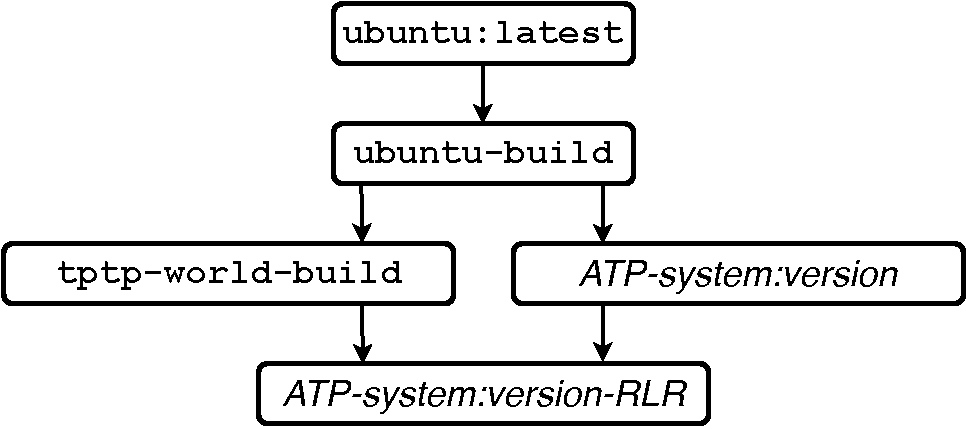
\includegraphics[width=0.8\textwidth]{ImageDAG} 
\caption{ATP System Container Hierarchy}
\label{ImageDAG}
\end{center}
\end{figure}

%--------------------------------------------------------------------------------------------------
\subsection{Creating ATP System Containers}
\label{BuildingATPSystemImages}

Each ATP system's {\em ATP-system-name}{\tt-build} is built on top of {\tt ubuntu-build}, and 
with {\tt tptp-world-build} forms the base for the final {\em ATP-system-name}{\tt -runsolver}.
{\em ATP-system-name}{\tt-build} adds the ATP system's executables to {\tt ubuntu-build}.
The ATP system is retrieved online, e.g., from a GitHub repository, and the necessary commands
to build the executables are run.
The executables are copied into the {\tt /artifacts} directory.
The choice of which version of the ATP system to containerize is made inside the {\tt Dockerfile},
e.g., in Figure~\ref{E---build} {\tt E 3.0.03} is chosen.
This localization is necessary because the incantations for selecting and retrieving an
particular ATP system version vary from system to system.
By convention the container is named {\em ATP-system-name}{\tt -build}, and by default has
the {\tt :latest} tag,
Figure~\ref{E---build} shows the {\tt Dockerfile} for E's {\tt -build}, using the command 
{\tt podman~build~-t~eprover-build~.}.

\begin{figure}[htb]
{\small
\begin{verbatim}
#------------------------------------------------------------
FROM ubuntu-build

# Clones repository
ARG E_VERSION=E-3.0.03
RUN git clone --depth 1 --branch $E_VERSION https://github.com/eprover/eprover.git

# Set working directory to cloned sources directory
WORKDIR /eprover

# Builds first-order executable
RUN ./configure --bindir=/artifacts && \
    make && \
    make install
# RUN cp PROVER/eprover /artifacts/eprover

# Builds higher-order executable
RUN ./configure --enable-ho && \
    make rebuild
RUN cp PROVER/eprover-ho /artifacts/eprover-ho
#------------------------------------------------------------
\end{verbatim}
}
\caption{The {\tt Dockerfile} for E's {\tt -build}}
\label{E---build}
\end{figure}

Each {\em ATP-system-name}{\tt -runsolver} is based on {\em ATP-system-name}{\tt-build} and 
{\tt tptp-world-build}. \jack{These -runsolver images *primarily* extend tptp-world-build and they are expected to only copy over what is necessary from their -build image. As such, if the prover requires a complicated environment (not just a simple static binary), their -runsolver dockerfile might need to duplicate a lot of the work they did in their -build image. This is because of the "AS" in the "FROM" line in the dockerfile.}
{\em ATP-system-name}{\tt -runsolver} adds the {\tt runsolver} utility to limit and report
the resource usage of the ATP system. \jack{Technically it doesn't. runsolver is added in tptp-world-build.}
Note how the containerization uses the default {\tt :latest} tagged 
{\em ATP-system-name}{\tt-build}. 
The executables from {\em ATP-system-name}{\tt -runsolver} are copied from its 
{\tt /artifacts} directory into this container's {\tt /artifacts} directory.
Additionally, the {\tt run\_system} script, described in Section~\ref{Running}, is copied into
{\tt /artifacts}.
By convention this container is named
{\em ATP-system-name}{\tt :}{\em ATP-system-version}{\tt -runsolver}, i.e., including the version
number so that users know what version of the ATP system has been containerized.
Figure~\ref{E---runsolver} shows the {\tt Dockerfile} for building E's {\tt -runsolver},
using the command {\tt podman~build~-t~eprover:3.0.03-runsolver~.}, i.e., it contains
E version {\tt 3.0.03}.

\begin{figure}[htb]
{\small
\begin{verbatim}
#------------------------------------------------------------
FROM eprover-build AS builder
FROM tptp-world-build

ENV PATH=".:${PATH}"
WORKDIR /artifacts

# E-specific stuff from ostensibly external image
COPY --from=builder /artifacts/eprover /artifacts/
COPY --from=builder /artifacts/eprover-ho /artifacts/

# run_image script 
ADD run_image /artifacts/

# run_E script 
ADD run_E /artifacts/

ENTRYPOINT ["runsolver"]
#------------------------------------------------------------
\end{verbatim}
}
\caption{The {\tt Dockerfile} for E's {\tt -runsolver}}
\label{E---runsolver}
\end{figure}

The {\em ATP-system-name}{\tt -runsolver} containers are pushed to {\tt dockerhub} in~\ldots\\
\hspace*{1cm}\href{https://hub.docker.com/repositories/tptpstarexec}{\tt hub.docker.com/repositories/tptpstarexec}\\
which has a directory for each ATP system.
The pushed containers are tagged as 
{\em ATP-system-name}{\tt :}{\em ATP-system-version}{\tt -runsolver-}{\em architecture},
where {\em architecture} is, e.g., {\tt arm64} or {\tt amd64}.
All the files for containerizing the ATP system are available from~\ldots \\
\hspace*{1cm}\href{https://github.com/StarExecMiami/starexec-kubernetes/tree/main/images}{\tt github.com/StarExecMiami/starexec-kubernetes/tree/main/images}\\
A {\tt Makefile} to containerize E, Leo-III, and Vampire is included.

%--------------------------------------------------------------------------------------------------
\subsection{Running ATP System Containers}
\label{Running}

A Python script {\tt run\_image.py} is available to run a containerized ATP system from the 
command line. \jack{Maybe "available to simplify and standardize running containerized ATP systems", since they could just be run using docker/podman directly.}
The script is shown in Appendix~\ref{runsystem}.
Minimally the script must have the {\em ATP-system-name}{\tt -runsolver} \jack{(image name)} as a command 
line argument.
By default {\tt run\_image.py} runs the {\em ATP-system-name}{\tt -runsolver} in a
{\tt podman} container, taking the problem from {\tt stdin}, imposing CPU and wall clock time 
limits of 60s, imposing no memory limit, with the intention that the ATP system should try prove 
that the problem's conjecture is a theorem.
The problem file is passed into the running container using Podman volume mounting, copying the
problem to the {\tt /artifacts/CWD/benchmark} file inside the container.
All the parameters can be changed via command line options to {\tt run\_image.py}.

The entrypoint in {\em ATP-system-name}{\tt -runsolver} is the {\tt runsolver} utility, 
which in turn starts the {\tt run\_system} script with the problem, CPU limit, wall clock limit, 
memory limit, and the proof request as arguments.
Each {\tt run\_system} script is responsible for starting the ATP system -- this action varies 
tremendously between ATP systems, and is thus usually provided by the system developer.
For example, E has its own script {\tt run\_E} that invokes the {\tt eprover} or {\tt eprover-ho}
binary depending on whether the problem is first-order or higher-order, and depending on the
intention passed in appropriate command line arguments are given to the selected binary along
with the problem file and time limit. \jack{Maybe it should be emphasized that run\_system wraps run\_E (that run\_E isn't an instance of the generic idea.)}

%--------------------------------------------------------------------------------------------------
\section{Towards a Cloud-native StarExec}
\label{StarExecK}

The term "cloud-native" has increasingly become synonymous with an approach to designing and operating applications that fully leverage the benefits of the cloud computing model.\footnote{For more information, one can refer to the initiatives led by the Cloud Native Computing Foundation (CNCF \url{https://www.cncf.io/}), which advocates for the adoption of this paradigm by fostering and sustaining an ecosystem of open source, vendor-neutral projects.}

Cloud-native applications are distinguished by their ability to scale more effectively, utilizing the cloud's capability to dynamically allocate resources. This development paradigm is closely aligned with DevOps practices, which emphasize collaboration between development and operations teams to automate the process of software delivery and infrastructure changes. It inherently supports infrastructure-as-code (IaC), a key DevOps practice, enabling the management and provisioning of infrastructure through code, which is both version-controlled and declarative.

Containers, as discussed in section \ref{Containerization}, play a pivotal role in cloud-native development. Also, so-called ``Dockerfiles,'' which specify the steps to create a container image, embody the declarative nature of IaC by detailing the desired state of a containerized application (and letting automated processes take care of synchronization). Similarly, Kubernetes YAML manifests, which define how applications run on Kubernetes, align with the IaC paradigm by allowing the entire deployment's specifications to be declared and managed as code.

The synthesis of these practices allows for the entire stack, from infrastructure to application, to be versioned, and automatically deployed as required. ATP users and developers can thus deploy StarExec (including its requisite infrastructure) in their preferred cloud environment or even in on-premises servers. This model offers unparalleled flexibility, scalability, and portability, free from the constraints of single vendors or platforms.
We thus advocate for an open distribution model that ensures that StarExec's infrastructure (``as code'') is readily accessible for modification and distribution (e.g., by cloning or forking from our GitHub repository). This approach significantly simplifies the process of utilizing state-of-the-art ATP technology, making it much more easily usable by anyone, anywhere.

\subsection{Re-engineering StarExec for the Cloud}

Recalling the current architecture of StarExec as discussed in section \ref{ContainerizingStarExec}, we have identified several areas for improvement to better serve our needs. Our ongoing efforts include:

\begin{enumerate}

\item \textbf{Utilization of containerized ATP systems} (see Section~\ref{ContainerizingATPSystems}), which will be hosted in a container registry (such as Docker Hub \url{https://hub.docker.com/}) instead of the current approach \dav{@Geoff/Jack: briefly describe how StarExec gets its provers right now}.

\item \textbf{Adding an abstraction layer for database communication} with the relational database (MariaDB) currently used to persist job information.  This layer will allow the database component to operate in its own container, significantly reducing coupling. Furthermore, by eliminating MariaDB-specific bindings, we enable compatibility with other database systems. This flexibility allows for seamless integration with existing SQL databases within the user's infrastructure, enhancing portability and adaptability.

\item \textbf{Transition to Kubernetes for cluster management}, thereby completely replacing the current cluster management system (SGE) with Kubernetes. This change offers numerous benefits: 

\begin{itemize}
	
	\item \textbf{Scalability:} Kubernetes excels at managing and scaling containerized applications, adapting to fluctuating workloads with ease. It also seamlessly integrates with most hardware provisioning tools, supporting many different public cloud platforms and on-premise frameworks.
	
	\item \textbf{Monitoring:} A vast array of observability tools (encompassing logging, metrics, tracing, etc.) support seamless integration with Kubernetes. Additionally, with its self-healing features, Kubernetes can automatically restart failed containers, replace and reschedule containers when nodes die, and kill non-responsive containers.
	
	\item \textbf{Efficiency:} Similar to SGE and other cluster management software such as Slurm and Torque, Kubernetes optimizes the use of underlying hardware by efficiently scheduling jobs and managing resources.
	
	\item \textbf{Flexibility:} Kubernetes' extensible architecture allows for custom schedulers and automated scaling decisions, enabling it to support a wide range of workloads, including stateless, stateful, and batch processing.
	
\end{itemize}
\end{enumerate}


Figure~\ref{ArchitectureK} shows the generic architecture of a future re-engineered StarExec system:

\begin{figure}[htb]
\begin{center}
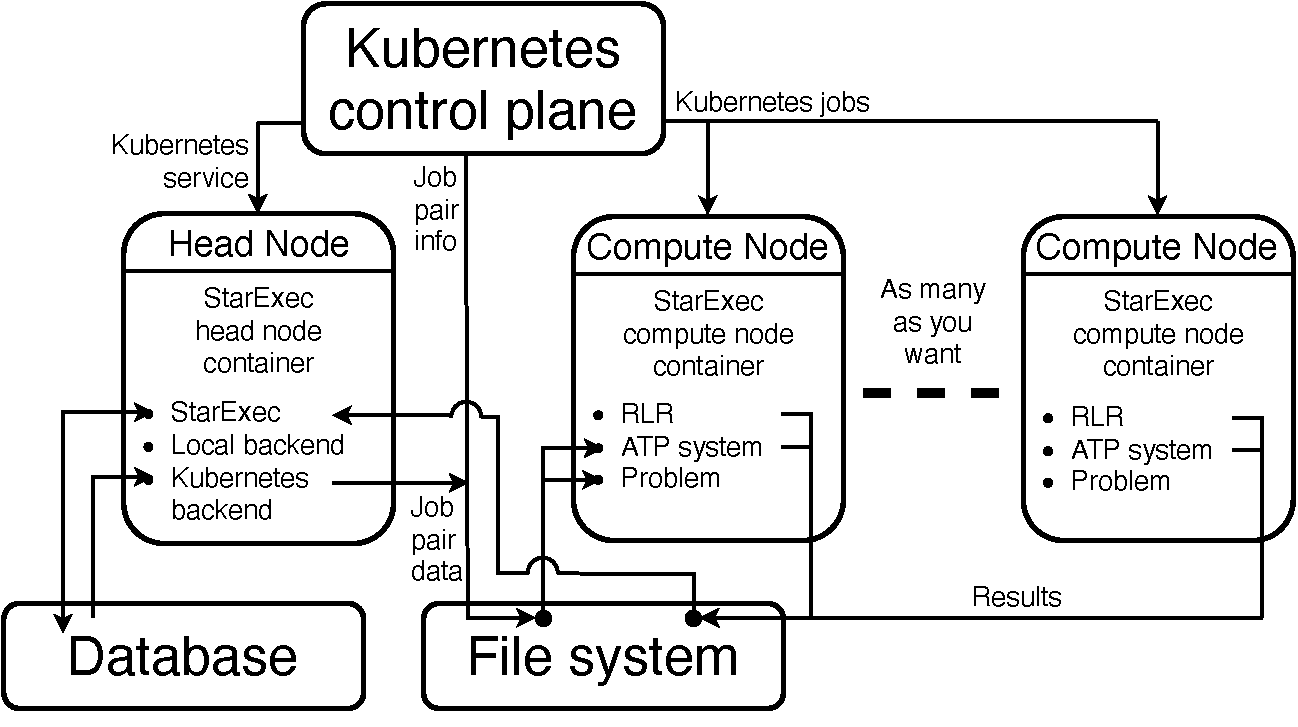
\includegraphics[width=0.8\textwidth]{ArchitectureK}
\caption{Architecture in Kubernetes}
\label{ArchitectureK}
\end{center}
\end{figure}

\subsection{Initial Deployment in AWS}

\dav{TODO}

An Amazon Research Award\footnote{%
Amazon Research Award, Fall 2023. Any opinions, findings, and conclusions or recommendations 
expressed in this material are those of the authors, and do not reflect the views of Amazon.} 
has been granted to implement StarExec with Kubernetes in AWS.
This instantiates the the generic implementation as follows:
\begin{packed_itemize}
\item The Kubernetes host will be Amazon Elastic Kubernetes Service (EKS)
\item The head and compute nodes will be Amazon EC2 nodes.
\item The database will be Amazon Relational Database (RDS).
\item The file system will be Amazon Elastic File System (EFS).
\item The ATP systems' containerization will be made compatible with (possibly be exactly) the 
      Amazon Trusted Solver (ATS) format.
\end{packed_itemize}

The entire migration of StarExec into AWS will be done using the ``infrastructure-as-code'' 
paradigm, using Amazon CloudFormation. 
The implementation will be tested by copying the TPTP community from StarExec Miami onto the 
new StarExec AWS.
Figure~\ref{ArchitectureAWS} shows the AWS-specific architecture.

\begin{figure}[htb]
\begin{center}
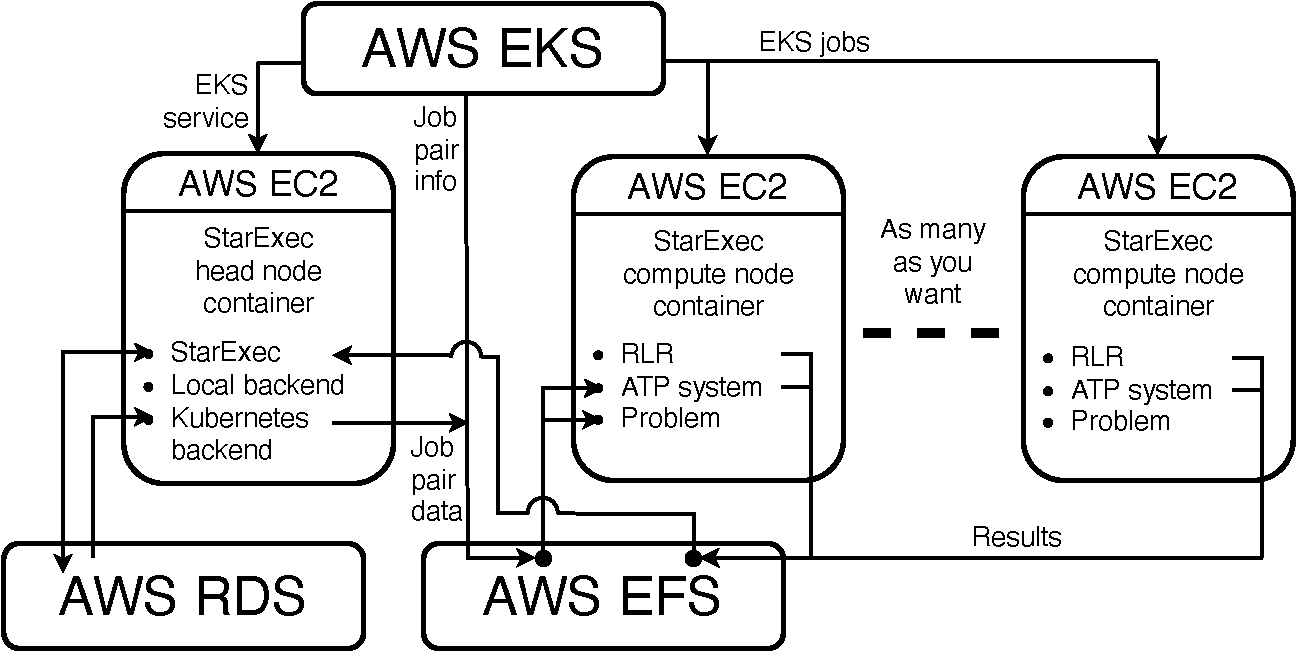
\includegraphics[width=0.8\textwidth]{ArchitectureAWS}
\caption{Architecture in EKS on AWS}
\label{ArchitectureAWS}
\end{center}
\end{figure}

%--------------------------------------------------------------------------------------------------
% Geoff
\section{Conclusion}
\label{Conclusion}

This paper has described work being done to containerize StarExec and ATP systems so that they 
can be run on a broad range of computer platforms.
Additionally, this work explains plans to build a Kubernetes backend in StarExec so that 
Kubernetes can be used to orchestrate distribute of StarExec job pairs over whatever compute 
nodes are available.

This is ongoing work -- some of the work is still ``in progress'', particularly embedding
StarExec in Kubernetes on AWS.
Hopefully the future will include StarExec being flexibly available in online compute clusters.

%--------------------------------------------------------------------------------------------------
\bibliographystyle{plain}
\bibliography{Bibliography.bib}
%--------------------------------------------------------------------------------------------------
\appendix

\newpage
\section{{\tt run\_image.py}}
\label{runsystem}
{\small
\begin{verbatim}
#--------------------------------------------------------------------------------
#!/usr/bin/env python3

import argparse
import subprocess
import os, sys
import shutil


def getRunsolverArgs(args):
    mem_part = f" -M {args.memory_limit}" if args.memory_limit > 0 else ""
    return "--timestamp --watcher-data /dev/null -C " + \
f"{args.cpu_limit} -W {args.wall_clock_limit}{mem_part}"


def getRunscriptArgs(args, args_format):
    parts = {
        'P': "/artifacts/CWD/benchmark",
        'C': args.cpu_limit,
        'W': args.wall_clock_limit,
        'I': args.intent,
        'M': args.memory_limit,
    }
    return ' '.join([str(parts[c.upper()]) for c in args_format])

def makeBenchmark(problem):
    if problem:
        shutil.copy(problem, "./benchmark")
    else:
        with open('./benchmark', 'w') as benchmark:
            benchmark.write(sys.stdin.read())


if __name__ == "__main__":
    parser = argparse.ArgumentParser("Wrapper for a podman call to a prover image")
    parser.add_argument("image_name", 
help="Image name, e.g., eprover:3.0.03-runsolver-arm64")
    parser.add_argument("-P", "--problem", 
help="Problem file if not stdin")
    parser.add_argument("--runscript", default="run_system PCWMI", 
help="System script and its args, e.g., 'run_E PWI', default=run_system PCWMI")
    parser.add_argument("-C", "--cpu-limit", default=60, type=int, 
help="CPU time limit in seconds, default=60")
    parser.add_argument("-W", "--wall-clock-limit", default=60, type=int, 
help="Wall clock time limit in seconds, default=60")
    parser.add_argument("-M", "--memory-limit", default=-1, type=int, 
help="Memory limit in MB, default=none")
    parser.add_argument("-I", "--intent", default="THM", choices=["THM", "SAT"], 
help="Intention (THM, SAT, etc), default=THM")
    parser.add_argument("--dry-run", action="store_true", 
help="dry run")
    args = parser.parse_args()

    # Format arguments
    runsolverArgs = getRunsolverArgs(args)
    runscript, runscriptArgsFormat = args.runscript.split()
    runscriptArgs = getRunscriptArgs(args, runscriptArgsFormat)

    # Construct podman command
    command = "podman run -v .:/artifacts/CWD -t " + \
f"{args.image_name} {runsolverArgs} {runscript} {runscriptArgs}"

    # Run command or print for dry run
    if args.dry_run:
        print(command)
    else:
        makeBenchmark(args.problem)
        subprocess.run(command, shell=True)
        os.remove("./benchmark")
#--------------------------------------------------------------------------------
\end{verbatim}
}
%--------------------------------------------------------------------------------------------------
\end{document}
%--------------------------------------------------------------------------------------------------
